\documentclass[11pt, a4paper, oneside]{report}
\usepackage[utf8]{inputenc}
\usepackage{graphicx}
\usepackage{hyperref}
\usepackage[acronym]{glossaries} % nomain
\makeglossaries
\usepackage[parfill]{parskip}
\usepackage{setspace}
\usepackage[numbers]{natbib}
\usepackage[titletoc]{appendix}
\graphicspath{ {images/} }
%\hyphenpenalty=10000
\pretolerance=10000
\tolerance=2000 
\emergencystretch=10pt


% CODE LISTINGS %
\usepackage{color}
\definecolor{editorGray}{rgb}{0.95, 0.95, 0.95}
\definecolor{editorOcher}{rgb}{1, 0.5, 0} % #FF7F00 -> rgb(239, 169, 0)
\definecolor{editorGreen}{rgb}{0, 0.5, 0} % #007C00 -> rgb(0, 124, 0)
\usepackage{upquote}
\usepackage{listings}
\lstdefinelanguage{JavaScript}{
  morekeywords={typeof, new, true, false, catch, function, return, null, catch, switch, var, if, in, while, do, else, case, break},
  morecomment=[s]{/*}{*/},
  morecomment=[l]//,
  morestring=[b]",
  morestring=[b]'
}

\lstdefinelanguage{HTML5}{
        language=html,
        sensitive=true, 
        alsoletter={<>=-},
        otherkeywords={
        % HTML tags
        <html>, <head>, <title>, </title>, <meta, />, </head>, <body>,
        <canvas, \/canvas>, <script>, </script>, </body>, </html>, <!, html>, <style>, </style>, ><
        },  
        ndkeywords={
        % General
        =,
        % HTML attributes
        charset=, id=, width=, height=,
        % CSS properties
        border:, transform:, -moz-transform:, transition-duration:, transition-property:, transition-timing-function:
        },  
        morecomment=[s]{<!--}{-->},
        tag=[s]
}

\lstset{%
    % Basic design
    backgroundcolor=\color{editorGray},
    basicstyle={\small\ttfamily},   
    frame=l,
    % Line numbers
    xleftmargin={0.75cm},
    numbers=left,
    stepnumber=1,
    firstnumber=1,
    numberfirstline=true,
    % Code design   
    keywordstyle=\color{blue}\bfseries,
    commentstyle=\color{darkgray}\ttfamily,
    ndkeywordstyle=\color{editorGreen}\bfseries,
    stringstyle=\color{editorOcher},
    % Code
    language=HTML5,
    alsolanguage=JavaScript,
    alsodigit={.:;},
    tabsize=2,
    showtabs=false,
    showspaces=false,
    showstringspaces=false,
    extendedchars=true,
    breaklines=true,        
    % Support for German umlauts
    literate=%
    {Ö}{{\"O}}1
    {Ä}{{\"A}}1
    {Ü}{{\"U}}1
    {ß}{{\ss}}1
    {ü}{{\"u}}1
    {ä}{{\"a}}1
    {ö}{{\"o}}1
}

\makeglossaries

% \makeatletter
% \defglsdisplayfirst[\acronymtype]{%
%   \firstacronymfont{#1}#4%
%     \protect\footnote{%
%       \glslink[\@gls@link@opts]{\@gls@link@label}{#3}: #2}}%
% \makeatother



\begin{document}
\newacronym[description={Real Time Protocol}]{rtp}{RTP}{Real Time Protocol}
\newacronym[description={Internet Engineering Task Force}]{ietf}{IETF}{Internet Engineering Task Force}
\newacronym[description={Hypertext Transfer Protocol}]{http}{HTTP}{Hypertext Transfer Protocol}
\newacronym[description={Hypertext Transfer Protocol Secure}]{https}{HTTPS}{Hypertext Transfer Protocol Secure}
\newacronym[description={World Wide Web Consortium}]{w3c}{W3C}{World Wide Web Consortium}
\newacronym[description={Synchronization Source Identifier}]{ssrc}{SSRC}{Synchronization Source Identifier}
\newacronym[description={Media Control Unit}]{mcu}{MCU}{Media Control Unit}
\newacronym[description={User Datagram Protocol}]{udp}{UDP}{User Datagram Protocol}
\newacronym[description={Session Description Protocol}]{sdp}{SDP}{Session Description Protocol}
\newacronym[description={Session Traversal Utilities for NAT}]{stun}{STUN}{Session Traversal Utilities for NAT}
\newacronym[description={Traversal Using Relays around NAT}]{turn}{TURN}{Traversal Using Relays around NAT}
\newacronym[description={Network Address Translator}]{nat}{NAT}{Network Address Translator}
\newacronym[description={Datagram Transport Layer Security}]{dtls}{DTLS}{Datagram Transport Layer Security}
\newacronym[description={Stream Control Transport Protocol}]{sctp}{SCTP}{Stream Control Transport Protocol}
\newacronym[description={Secure Real-time Protocol}]{srtp}{SRTP}{Secure Real-time Protocol}
\newacronym[description={Interactive Connectivity Establishment}]{ice}{ICE}{Interactive Connectivity Establishment}
\newacronym[description={Web Real-Time Communication}]{wrtc}{WebRTC}{Web Real-Time Communication}
\newacronym[description={Real-time communication}]{rtc}{RTC}{Real-time communication}
\newacronym[description={JavaScript Session Establishment Protocol}]{jsep}{JSEP}{JavaScript Session Establishment Protocol}
\newacronym[description={Web Real-Time Communications}]{rtcweb}{RTCWeb}{Web Real-Time Communications}
\newacronym[description={Universal Plug and Play}]{upnp}{UPnP}{Universal Plug and Play}
\newacronym[description={Transmission Control Protocol}]{tcp}{TCP}{Transmission Control Protocol}
\newacronym[description={Session Initiation Protocol}]{sip}{SIP}{Session Initiation Protocol}
\newacronym[description={Session Border Controller}]{sbc}{SBC}{Session Border Controller}
\newacronym[description={Demilitarized Zone}]{dmz}{DMZ}{Demilitarized Zone}
\newacronym[description={VoIP}]{voip}{VoIP}{Voice over IP}
\newacronym[description={Session Description Protocol Security Descriptions}]{sdes}{SDES}{Session Description Protocol Security Descriptions}
\newacronym[description={Software development kit}]{sdk}{SDK}{Software development kit}
\newacronym[description={Bring your own device}]{byod}{BYOD}{Bring your own device}
\newacronym[description={Central Processing Unit}]{cpu}{CPU}{Central Processing Unit}
\newacronym[description={Application programming interface}]{api}{API}{Application programming interface}
\newacronym[description={Acoustic Echo Cancellation}]{aec}{AEC}{Acoustic Echo Cancellation}
\newacronym[description={IP Multimedia Subsystem}]{ims}{IMS}{IP Multimedia Subsystem}

% TITLE %
\author{H\aa vard A. Heggheim\\[1cm]
Supervisors: Lars Petter Helland \&\\ Anders Øvreseth}
\date{\today}

\title{\vspace{-4cm}{
 {\huge Interworking WebRTC with Enterprise Multimedia Communications}\\[0.4cm]
 {\large Bergen University College and University of Bergen}\\
 {\large Joint Master's Programme in Software Engineering}\\[1cm]
 {\vspace{+5cm}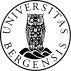
\includegraphics[height=3cm]{uiblogo.png}}
 {\hspace{+2cm}
\includegraphics[height=3cm]{ny_hib_logo.jpg}}
 \vspace{+4cm}
}}

\maketitle

% INTRO %
\newpage
\pagenumbering{roman}
\setcounter{page}{1}
\newpage
\thispagestyle{empty}
%!TEX root = ../main.tex

page 211
state research problem
announce key themes
state the main point or launching point that anticipates the main point

context+problem+main point

put in key search words

\begin{abstract}
% The use of communication technologies today consume a large time of our daily lives. A lot of these technologies are now moving to Internet based solutions. Some of these services are collaboration tools that do video/audio and application sharing. This thesis will look at streaming media on the web in a collaborative enterprise environment. There are currently many Internet based communication services existing today that does this, but most of these are not open, cost money and require the installation of a plugin. This thesis will look at how Visual Solutions can integrate the new WebRTC APIs for doing real-time streaming of media in the browser with their current visual collaboration solution Virtual Arena.

% The aim of this thesis is to find the most suitable way for Visual Solutions to implement live media sharing in the web browser with their current application Virtual Arena. The goal is to detect challenges and problems that might occur with the use of the new Web APIs.

% The HTML5 standard introduces many new APIs that give web browsers the ability to communicate directly with each other in real-time. But there are many solutions and the different providers doesn't seem to agree on a single solution. This thesis will examine using these new APIs to see how we can integrate the browser in current media collaboration systems. The goal being to determine the feasability of using these new APIs and evaluate their usage. This thesis hopes to aid in developing solutions for media sharing in the browser that can be used in an enterprise setting.
\end{abstract}


This is a study on how to integrate \gls{rtcweb} with a enterprise communication system. Each system is broken down into several components on the transport level. A gateway model interoperating between the two architectures are created and then evaluated by looking at similar systems.

\\gls{rtcweb} is defined as the underlying technologies of a set of APIs drafted by the \gls{w3c} as \gls{webrtc}. It supports browser-to-browser applications for audio/video chatting without plugins. \gls{wrtc} is currently seeing great support with two of the major browser vendors; namely Google and Mozilla. Both Apple and Microsoft currently lag a bit behind, but they are both active in the working groups that define the standards. A ton of new companies are appearing using this new technology because of the easy entry these APIs provide. The browser APIs are simple to use and let's you basically create your own phone company over a weekend. This has turned the eye of bigger telecom vendors like Cisco and Ericsson. All of them are looking into how they can use \gls{wrtc} in the future. One of the greatest advantage of utilizing \gls{wrtc},% is the whole range of new devices you suddenly have access to. Using the optimized audio and video engine of \gls{rtcweb}, you can scale for pretty much any device that has support for the latest Chrome or Firefox browser. The integration of \gls{wrtc} allows for easier adopting of the \gls{byod} to work policy that permits employees to bring their personally owned mobile devices (laptops, tablets, and smart phones) to work. The problems of using a mobile \gls{wrtc} client within an enterprise setting is discussed in this thesis.  

Using guidelines derived from looking at different ways of doing this integration, in order to aid in deciding if this is a feasible way to go about getting support for mobile devices in current enterprise systems. The use of a gateway outlined in this thesis is the main topic together with recommendations for implementing a mobile \gls{wrtc} client for tablets and smartphones.

\newpage
\thispagestyle{empty}

\renewcommand{\abstractname}{Acknowledgements}
\begin{abstract}

This paper is written in collaboration with Visual Solutions.

I would like to thank my supervisor Lars-Petter Helland from Bergen University College for guidance and support.
Second, I would like to thank Anders Øvreseth from Visual Solutions for the opportunity to do this thesis and for answering questions.
Supervisor: Lars-Petter Helland

\end{abstract}

\newpage
\thispagestyle{empty}
\setcounter{tocdepth}{3}
\tableofcontents

\newpage
\thispagestyle{empty}
\listoftables

\newpage
\thispagestyle{empty}
\listoffigures

\newpage
\thispagestyle{empty}
\printglossaries

% MAIN SECTION %
\newpage
\onehalfspacing
%\setlength{\parindent}{1cm}
\pagenumbering{arabic}
\setcounter{page}{1}
\chapter{Introduction}
We live in a world where communication plays a major role in how we conduct business. Location independant work roles are more common now than ever before. Two persons no longer have to sit next to each other in order to collaborate on a project, they just need good real-time communication tools. There are several methods of doing communication, including: web-based communication, video conferencing, e-mails, telephoned meetings and forum boards. In may 2011, Google released an open-source project for browser-based real-time communication known as \gls{wrtc}\cite{google-release-of-webrtc}. There is an ongoing effort to standardise this work. The term \gls{wrtc} is usually used in general to cover all aspects of this technology, however specifically the underlying protocols and codecs are defined as \gls{rtcweb} and is standardised by the IETF\cite{ietf}. \gls{wrtc} actually only covers the browser APIs defined by the W3C\cite{w3c}. These APIs are integrated directly in the browser and allows smaller enterprises to create advanced communication applications in a much simpler way than ever before. These new APIs has the advantage of being able to work on every single device that runs a \gls{wrtc} compatible web browser. By integrating \gls{rtcweb} into older communication systems, we allow these systems to interact with a whole range of new devices. By modeling a bridge between \gls{wrtc} and enterprise communication systems, we can reach these devices without having to modify or break current system architecture.

Large companies like Cisco and Microsoft are big players in the communications industry. They sell tools that makes us able to communicate in real-time. These tools are expensive and generate a lot of revenue for these companies, but now we see a rise of smaller enterprises taking market shares in certain areas from these big companies. These enterprises are efficient at using new technologies that simplifies greatly the way we can develop communication applications. \gls{wrtc} is one of these new technologies. It is directly integrated in the web browser, so that we can use simple web APIs to handle communication between peers. All the advanced underlying technologies of doing transportation of media, routing the traffic through firewalls, and dynamically adjusting bandwidth usage, is taken care of by the browser. Using these new simple APIs we can quickly develop advanced communication systems, and since they are integrated directly in the browser, it is also possible to get mobile device support with a lot less effort than before. The main problem here is that this technology does not have any way of communicating with older communication systems. This is a problem for companies that want to take advantage of the new possibilites this technology provides, such as mobile support for almost all platforms that can run a web browser.

In collaboration with the company Visual Solutions\footnote{http://www.bbvisuals.com/} I will look at how we can integrate an older communication system with the new \gls{wrtc} technology. This work could be of benefit to all communication companies that want's to take advantage of the new possibilities that \gls{wrtc} provides. Visualize yourself getting late to a meeting, with a simple click on a link you got in an invitation, you will be able to participate in the meeting from your mobile device, wherever you are with an internet connection, this would be possible. Visual Solutions have created an application called Virtual Arena that does collaboration between peers thorugh sharing of audio, video, and applications. This application will be used as a reference of a typical enterprise communication system.

This thesis will model a solution to bridge \gls{wrtc} with a typical enterprise desktop communication system. I do this by going through all the tehnologies that \gls{wrtc} requires to be implemented for a connection between two peers to occur. Looking at different ways of creating a gateway between two systems, I will suggest an architecture with all the components required for making the interaction. I will also focus especially on the communication between mobile devices, as this is one of biggest advantages of utilizing \gls{wrtc}.

This thesis will begin by giving an introduction to \gls{wrtc} and basic transportation protocols. To understand how \gls{wrtc} works you need to understand a lot of new concepts. These will be described in the background chapter. Then I will describe in detail what the main problems of bridging \gls{wrtc} with a desktop enterprise communication system are. I will then model a gateway that makes communication between \gls{wrtc} and Virtual Arena possible. I will also look at different problems that needs to be handled when developing a mobile \gls{wrtc} client. Lastly I will take a look into the future and make a prediction of what new features will soon be available for \gls{wrtc}.

\chapter{Background}
%!TEX root = ../main.tex

This chapter will explain the background for this thesis, starting with the introduction of Visual Solutions and their practical problem. Secondly I will introduce the RTCWeb technologies and WebRTC browser APIs. Lastly I will look at the use of \gls{wrtc} on mobile devices.% look at similar technologies, and lastly look at current use cases and implementations of \gls{wrtc}.

\section{Enterprise collaboration systems architecture}

This section will first introduce the company Visual Solutions\footnote{http://www.bbvisuals.com/} who provided the practical problem. Secondly I will give a quick overview of how the application Virtual Arena works by describing its underlying architecture, then I will look at how the enterprise firewall works, and lastly look some of the security concerns that occur when a enterprise collaboration system has to access the public internet.

\section{Visual Solutions}
Visual Solutions is a Norwegian company in the BB Visual Group\footnote{http://www.bbvisualgroup.com/}. Their primary business is within the integration of operations for the oil and gas industry. They create solutions enabling collaboration across organisation units and geographic locations. One of their applications Virtual Arena\cite{solutions_b2_virtual_2014}, which from now on will be referred to as VA, is a powerful and interactive tool that allows for high-performance application sharing, with audio and video communication from a 3D shared scene\ref{fig:?}. VA supports many-to-many collaborative scenarios by utilizing a media server which will be described in the next section. 

\section{Virtual Arena}
VA is the application that Visual Solutions has created for doing visual collaboration\cite{VirtualArena} over IP. The architecture of VA is visualized in Figure\ref{?}. The application uses a media server that serves multiple purposes. It acts as a \gls{mcu}, applies mitigation strategies for scenarios with limited bandwidth, and also sharing of applicaton data. Mitigation strategies can f.ex be reducing the video bitrate to adjust adapt for a poor connection. The media server works together with a router for distributing the streams. By utilizing a media server VA can support a lot incoming and outgoing streams. A client can subscribe to multiple streams of audio/video and applications. It manages these connections using a tree structure, but this is an advanced topic that I won't go into detail about. In the next subsections the different parts of the architecture\ref{?} will be described with the necessary information required to understand the practical problem this thesis will try to solve. 
\\
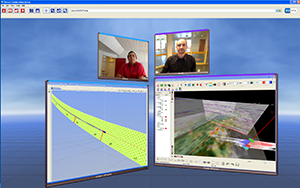
\includegraphics[scale=0.6]{virtualarena.png}
\\
\\

\subsection{Signaling}
VA has a proprietary way of doing signaling over RTCP. RTCP is control protocol for RTC. This is where the clients send messages to the media server describing which streams they want to subscribe to. Communication between peers and the media server is done by opening up ports in the firewall to listen for incoming TCP and UDP connections. These ports are preconfigured for the application. The media server can receive incoming streams and route it to all peers connected. The streams are identified using a SSRC, which is defined in the header packets of the RTP streams.

\subsection{Transport layer}
VA uses raw RTP stream over UDP. This is basically the most standard protocol used for transmitting real-time data in enterprise communication systems\cite{}.

\subsection{Media}
VA uses free and open source codecs for audio and video. It uses Speex for audio, and Theora for video. These are not the most commonly used codec, as the g.711 for audio and H.264 for video are the most common ones. Even though H.264 is licensed by Ericsson, it offers the added benefits of hardware acceleration in a lot of graphic cards, and is also one of the best codecs for real-time streaming as of now\cite{source}.

%%are common in, but h.264 g.711 standard in ims systems%%

\subsection{Security}
VA only uses raw UDP streams because nothing more is needed. It operates in a closed business environement, so transport level encryption is not needed, because unidentified peers are not allowed inside the network anyways. The enterprise firewall has very strict policys, only allowing certain kinds of traffic.?????

\subsection*{Summary}
VA operates like a typical enterprise comunication system. CODEC?? 

\newpage
\section{Introduction to RTCWeb and WebRTC APIs}

\gls{wrtc} is a collection of standards, protocols, and Javascript APIs. The combination of these enables web browsers to do peer-to-peer audio, video and data sharing between browsers. There is no plugin or third-party software required. Real-time communication is now becoming a standard feature in browsers that any web site can use via simple APIs. Delivering functionality such as live audio and video sharing and data exchange requires a lot of new processing capabilities in the browser. We will look at the underlying technologies and protocols of \gls{wrtc}, such as audio and video processing, transportation of media, and security. These technologies are abstracted behind three primary browser APIs:

\newpage
\begin{itemize}
\item MediaStream: capturing audio and video streams
\item RTCPeerConnection: communication of audio and video data
\item RTCDataChannel: communication of arbitrary application data
\end{itemize}

With the above APIs you can: capture media from a camera on your device, do peer discovery, connection negotiations, real-time transportation of media and sharing of arbitrary data. But first of all we look at the working groups behind the development of \gls{wrtc}.

\subsection{Standards and development}
The \gls{wrtc} architecture consists of different standards, covering both protocols and browser APIs:

\begin{itemize}
\item All the different protocols and data formats required to make \gls{wrtc} work is defined by the IETF Working Group \gls{rtcweb}. They are responsible for defining protocols, data formats, security, and all other aspects to enable peer-to-peer communication in the browser.
\item The \gls{wrtc} \gls{w3c} Working Group is responsible for defining the browser APIs.
\end{itemize}

WebRTC is the first open standard to tranport data over \gls{udp} in the browser. However doing this requires a lot more than raw \gls{udp} to do real-time communication, we need media processing and added security layers.

\subsection{Audio and video}
Doing live audio and video sharing requires processing to enhance image quality, doing synchronization, echo cancellation, noise reduction and packet loss concealment\cite{grigorik_high_2013}. On the transmitting end the bitrate must be adjusted to fluctuating bandwidth and latency between clients. On the receiving end the client must decode the streams in real-time and be able to adjust network jitter and latency delays. These are complex problems, but WebRTC includes fully featured engines in the browser, which takes care of all the signal processing for us. All of the processing is done directly by the browser.

\begin{figure}[here]
\centerline{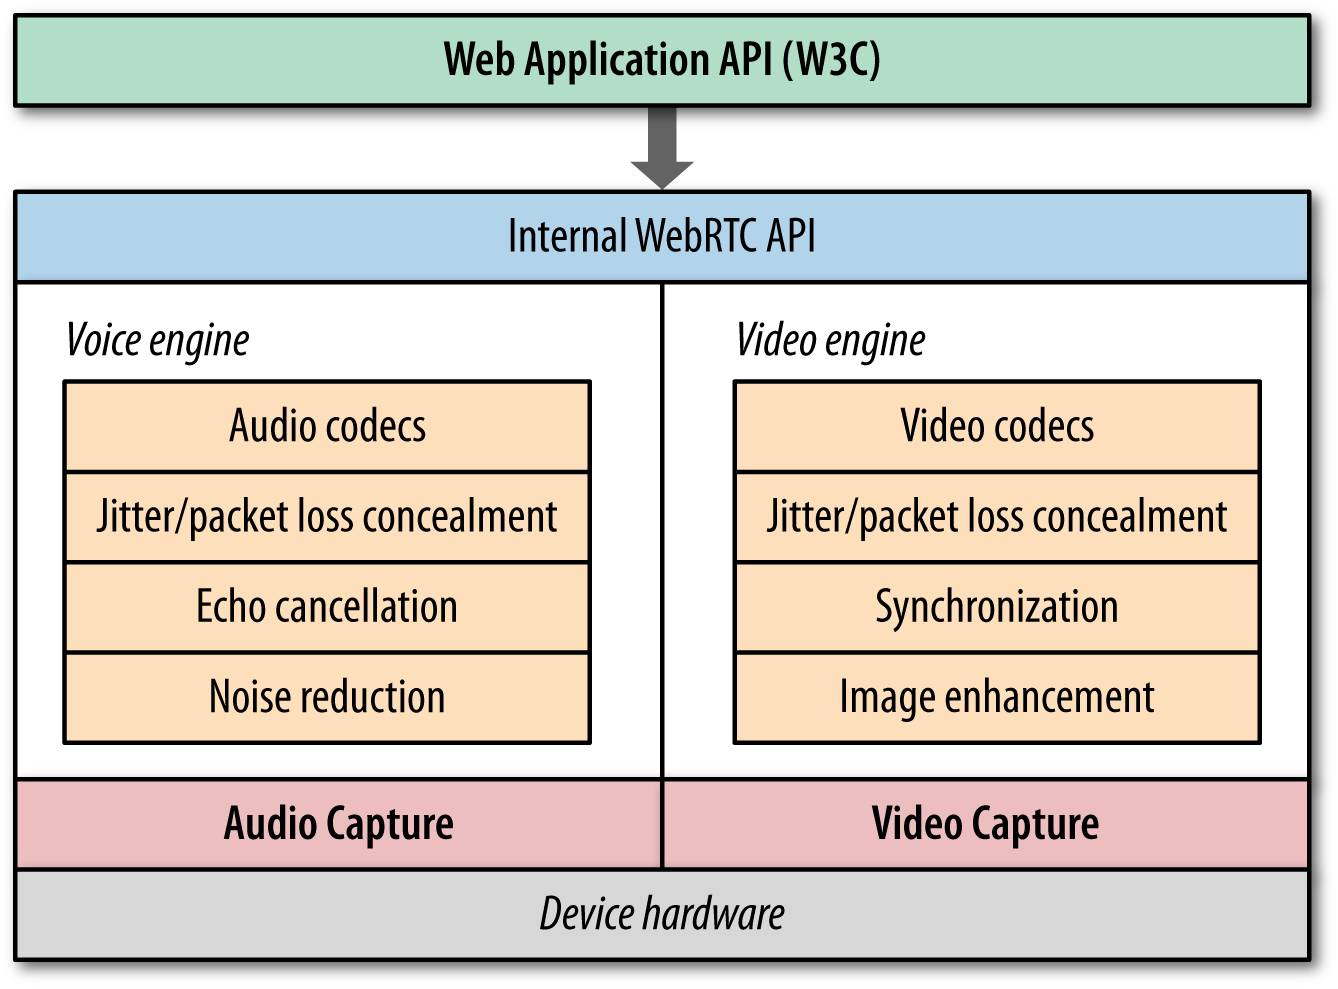
\includegraphics[scale=0.8]{audiovideocapture.png}}
\caption{WebRTC audio and video engines}
\label{fig:audiovideocapture}
\end{figure}

\subsection{Real-time transports}
When it comes to real-time communication, synchronization and low latency is more important than reliability. This is the reason why the \gls{udp} protocol is preferred for doing real-time communication. While \gls{tcp} delivers a reliable communication, there can be delays. If a packet is lost, it is re-requested. The human brain does't handle latency in communication very well, but we are good at filling in the gaps. Therefore we use UDP, which is a connectionless solution. It doesn't check the state of the message. So part of the message could be lost, and we wouldn't know, but the connection would run without delay.

\gls{udp} is the foundation for doing real-time communication, but to meet all the specified requirements of \gls{wrtc}, we need to support a lot of protocols and services on top of that.

\begin{figure}[here]
\centerline{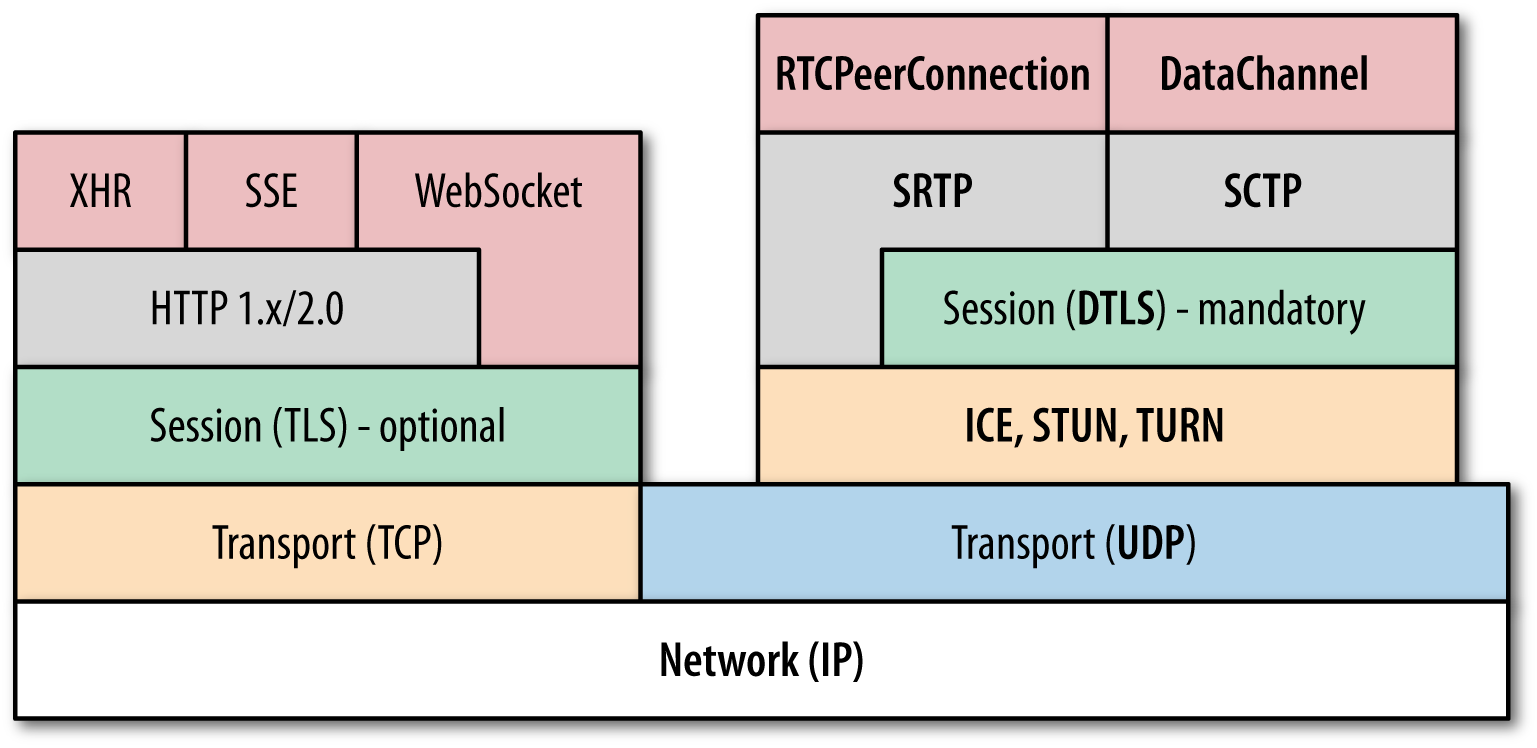
\includegraphics[scale=0.8]{wrtc-protocol-stack.png}}
\caption{WebRTC protocol stack}
\label{fig:wrtc-protocol-stack}
\end{figure}

\gls{ice}, \gls{stun}, and \gls{turn} are needed to establish a connection over \gls{udp} in \gls{wrtc}. Encryption is mandatory and \gls{dtls} is used to secure all transfers between peers. \gls{srtp} and \gls{sctp} are used to multiplex the different streams, provide congestion and flow control, and provide delivery on top of \gls{udp}.

After looking at the underlying technologies of \gls{wrtc} defined as RTCWEB, we will now give an introduction to the drafted browser browser APIs. We are only going to introduce the first two of them, since the third one is not applicable to this project.

\subsection{getUserMedia()}
Acquiring audio and video is done by using JavaScript APIs that enables the browser to acquire audio and video from a physical device such as a webcam or microphone. Incoming streams from remote network peers are also captured and everything is packaged in a MediaStream object. Inside the MediaStream object we have one or more individual tracks that are synchronized with one another. The output can be sent to a local audio or video element, post-processing scripts or remote peers.

The MediaStream object represents a real-time media stream and allows the application to manipulate individual tracks and specify outputs.


The getUserMedia() API allows us to specify a list of mandatory constraints to match the needs of the applicaton:

\lstset{language=Javascript} 
\begin{lstlisting}
var constraints = {
	audio: true,
	video: {
		mandatory: {
			width: { min: 1280 },
			height: { min: 720 },
			frameRate: 30
		},
		optional: []
	}
}

navigator.getUserMedia(constraints, stream, error);
\end{lstlisting}

Once a stream is acquired we can feed them into other APIs such as Web Audio for enabling advanced audio processing. Canvas API for post-processing video frames and WebGL can apply 3D effects on the output stream.

Simplified the getUserMedia() is an API to acquire audio and video streams. The media is automatically optimized, encoded and decoded by the audio and video engines. Then we can display the media locally in an audio or video element in the browser.


\subsection{RTCPeerConnection}
The RTCPeerConnection is responsible for managing the peer-to-peer connection. It uses an \gls{ice} Agent for NAT traversal, keeps track of streams, and triggers renegotiation when required. It provides an API for generating offer and answer.

To be able to understand RTCPeerConnection we need to understand signaling and \gls{ice}.

\subsubsection{Establishing a connection}

\begin{figure}[here]
\centerline{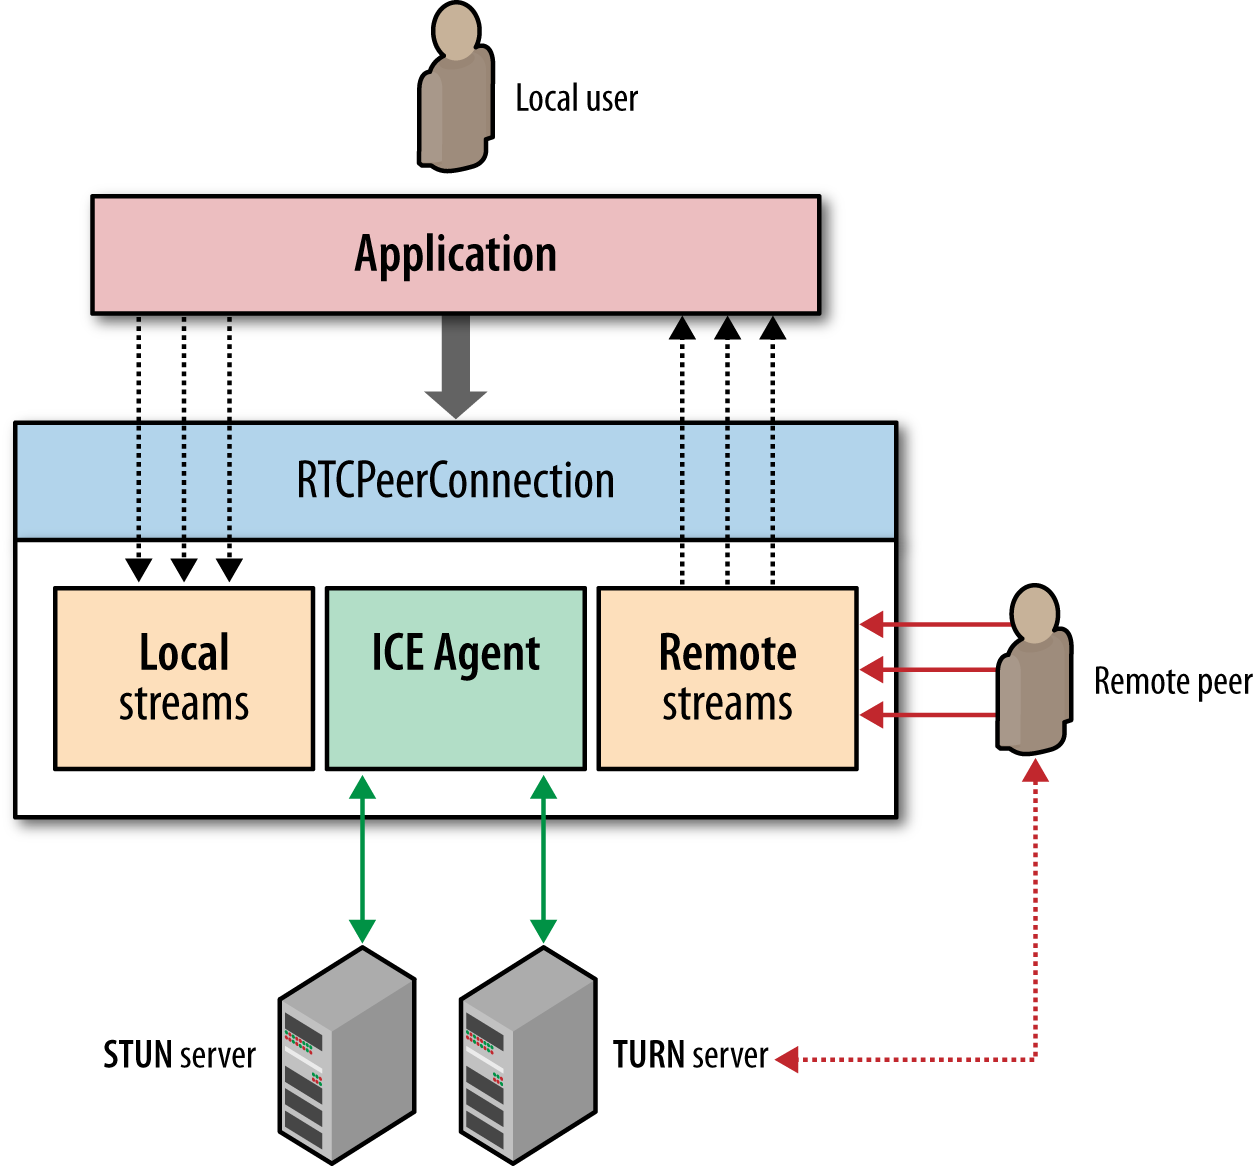
\includegraphics[scale=0.8]{peerconnection.png}}
\caption{RTCPeerConnection API}
\label{fig:rtcpeerconnection}
\end{figure}

\begin{enumerate}
\item Input devices are opened for capture as the media source. This is done using the getUserMedia API.
\item Now we have to signal the other users that we want to connect to them. using RTCPeerConnection we send an \gls{sdp} offer to the other clients, which generates an \gls{sdp} Answer. The \gls{sdp} here includes \gls{ice} candidates,  which allows for firewall traversal.

\begin{figure}[here]
\centerline{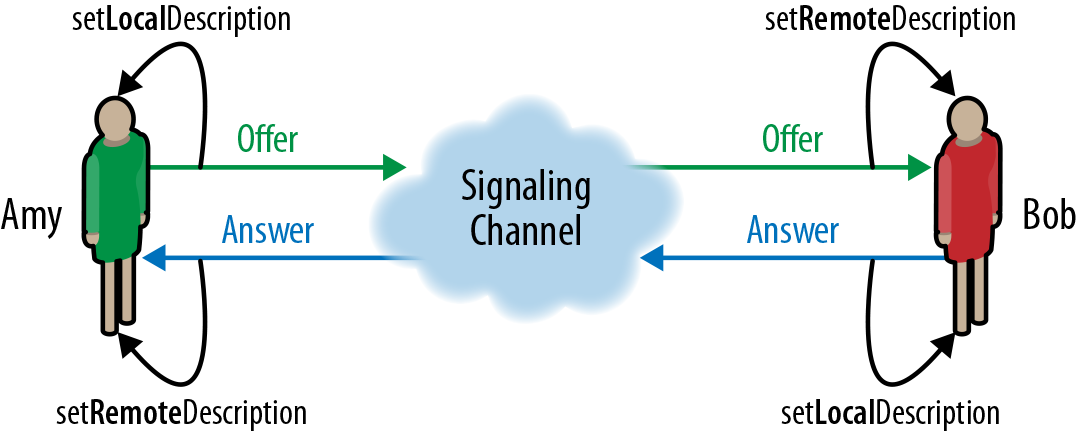
\includegraphics[scale=1.0]{SDPexchange.png}}
\caption{Offer/answer SDP exchange between peers}
\label{fig:sdp-exchange}
\end{figure}

\item Once connection is successful, a \gls{dtls} connection is opened and all the media from input devices are encoded into packets and transmitted using \gls{srtp}-\gls{dtls} streams.
\item At the destination, the packets are decoded and formatted into a MediaStream.
\item The MediaStream is sent to output devices
\end{enumerate}


\subsubsection{Signaling}
While \gls{wrtc} does all the routing and connectivity check for us with the \gls{ice} protocol, we have to do session negotiation ourselves. To do this we must extend an offer to the receiving peer and we need an answer in return. Choice of signaling application is up to us. The \gls{wrtc} standard does not define a signaling protocol, but the key information that needs to be exchanged is the \gls{sdp}, which specifies the necessary transport and media configuration information necessary to establish a connection. This approach is outlined by \gls{jsep}. Assuming we have a shared signaling channel, we can initiate a \gls{wrtc} connection.


\begin{lstlisting}
var signalingChannel = new SignalingChannel();
var pc = new RTCPeerConnection({});

navigator.getUserMedia(constraints, onStream, error);

function onStream(stream) {
  pc.addstream(stream);

  pc.createOffer(function(offer) {
    pc.setLocalDescription(offer);
    signalingChannel.send(offer.sdp);
  });
}
\end{lstlisting}


\subsubsection{SDP}
\gls{wrtc} uses a \gls{sdp} to describe the parameters of a connection. It represents a list of properties describing the connection, ICE candidates, \gls{dtls} parameters, types of media, codecs, bandwidth, \gls{ssrc}s and other metadata information\footnote{http://tools.ietf.org/id/draft-nandakumar-rtcweb-sdp-01.html}.



Here is some of the information that is generated after a call createOffer() has generated the \gls{sdp} description:

\begin{lstlisting}[frame=single]
...snip...
m=audio 1 RTP/SAVPF 111 103 104 0 8 106 105 13 126
c=IN IP4 0.0.0.0
a=rtcp:1 IN IP4 0.0.0.0
a=ice-ufrag:fAYfQM/iWMQPqiHs
a=ice-pwd:pgbuPPRdpKq+obC0lyRxVDe/
a=extmap:1 urn:ietf:params:rtp-hdrext:ssrc-audio-level
a=rtpmap:111 opus/48000/2
a=maxptime:60
a=ssrc:2209464108 cname:7oIEPieg3XZzHJdN
a=ssrc:2209464108 mslabel:uWu6kVvHhYbbkOtNalf5E2LFgjx4cpGMhnfo
a=ssrc:2209464108 label:2b626a18-c54c-4c1b-9f42-03519a9b63f2
m=video 1 RTP/SAVPF 100 116 117
...snip...
\end{lstlisting}


\subsubsection{ICE}
In order to establish a peer-to-peer connection, the peers must be able to send packets to each other. This is easy when you know which ip and port to listen to for incoming messages, but hard when you don't know. Normally there would be firewalls and NAT devices between most peers. In a local environment where there is no firewall, we could establish a connection between two peers by appending the IP and port number to the \gls{sdp}, and forward it to the other peer. What \gls{ice} does is getting around these restrictions by doing connectivity checks and route planning between peers. \gls{ice} gathers all possible addresses it can in address:port and transport triplets\cite{ivov_ice_2013}. \gls{ice} calls these `candidates', and once candidates have been gathered, they are ordered in a list based on priority. Highest priorities are assigned to candidates with the least overhead: those that you get from the device itself, the IP `host' candidates. Next in line are STUN candidates, which are f.ex obtained via \gls{upnp}. Finally the `relayed' candidates that is obtained from TURN servers come. By relaying media through a TURN server, we no longer have a peer-to-peer connection, this is costly and not something we want to do unless there is no other way of connecting to each other.

\subsubsection{Secure communication}
Once we have completed the \gls{sdp} anwers and offers, and traversed NATs, we have come a long way. But \gls{wrtc} require that we encrypt all communication. On top of \gls{udp}, we have \gls{srtp} used for transporting media securely, and \gls{dtls} which is used to negotiate secret keys for encrypting media data. This all taken care of by \gls{wrtc}, and once we have everyting else in place, we are ready to establish peer-to-peer connections.

\subsubsection{Bringing it all together}
To summarize the process of creating a peer-to-peer connection:

\begin{lstlisting}
<video id='local' autoplay></video>
<video id='remote' autoplay></video>

<var ice = {"iceServers": [
    {"url": "stun:stunserver.com:12345"},
    {"url": "turn:turnserver.com", "username": "user", "credential": "pass"}
  ]};

  var signalingChannel = new SignalingChannel();
  var pc = new RTCPeerConnection(ice);

  navigator.getUserMedia({ "audio": true, "video": true }, onStream, logError);

  function onStream(evt) {
    pc.addStream(evt.stream);

    var localVideo = document.getElementById('localVideo');
    localVideo.src = window.URL.createObjectURL(evt.stream);

    pc.createOffer(function(offer) {
      pc.setLocalDescription(offer);
      signalingChannel.send(offer.sdp);
    });
  }

  pc.onicecandidate = function(evt) {
    if (evt.candidate) {
      signalingChannel.send(evt.candidate);
    }
  }

  signalingChannel.onmessage = function(msg) {
    if (msg.candidate) {
      pc.addIceCandidate(msg.candidate);
    }
  }

  pc.onaddstream = function (evt) {
    var remoteVideo = document.getElementById('remoteVideo');
    remoteVideo.src = window.URL.createObjectURL(evt.stream);
  }

  function logError() { ... }
</script>
\end{lstlisting}

\begin{enumerate}
\item{Initialize a shared signaling channel}
\item{Initialize a PeerConnection Object}
\item{Acquire local media streams}
\item{Register local media streams with PeerConnection}
\item{Gather ICE candidates and generate SDP offer describing connection and send to peer via the signaling channel}
\item{Register remote ICE candidates and initiate connection}
\item{Receive remote media stream}
\end{enumerate} 


\subsection{Summary}
We have now looked at the underlying aspects of \gls{wrtc} and the subsequent browser APIs. We know that there are two different working groups: IETF working on the protocols and W3C working on the browser APIs. We also know how to initiate a simple peer-to-peer connection. In the next chapter we will look at some of the challenges of utilizing \gls{wrtc} on a mobile device.

\newpage
\section{Mobile devices}
%!TEX root = ../main.tex

The use of mobile broadband for accessing the Internet via tablets and smartphones has increased rapidly as a result of high speed mobile networks becoming more available such as 3G and 4G. The web browser on these devices are becoming more and more similar in capabilities to their desktop versions. It is possible to run \gls{wrtc} applications in some of them, and these features will become more available with time. This section is going to look at the use of \gls{wrtc} in mobile devices. We start by looking at some of the issues we have to deal with when working with mobile devices, then we will look at performance and quality metrics derived from current research.

\subsection{Network performance}
It is feasible to run \gls{wrtc} applications on mobile devices. However, battery consumption,  persistent connectivity, and quality performance remain a big challenge. A lot of work is being done in radio technologies, but the most important factor is how the applications, protocols, and API's are designed\cite{isomaki2012considerations}. First we will look at some of the performance issues of serving wireless video.

The most used and relevant networks are Wi-Fi, WiMAX, and the different telecommunication networks. Serving wireless video is a significant challenge for already-stressed cellular data networks\cite{erman2011over}. Video traffic requires high bandwidth, imposes latency and packet loss. The key is to deliver video as high in quality as the network supports. By looking at a study testing video and audio quality on two differenet WiMAX networks\cite{fund2013performance}, we can see variations of performance in two different locations.

\pagebreak
\begin{figure}[here]
\centerline{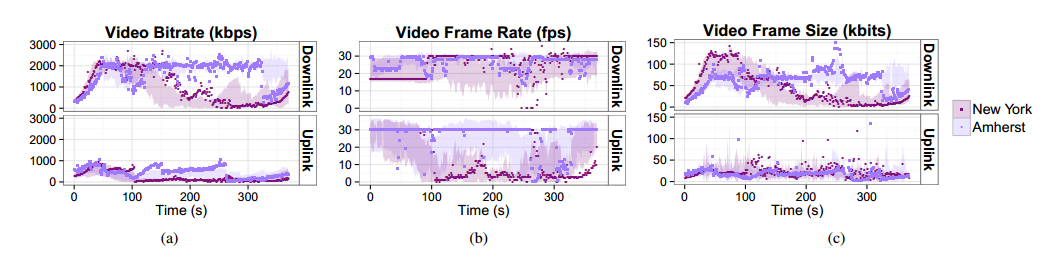
\includegraphics[scale=0.4]{mobile-video-metrics.png}}
\caption{WebRTC video performance. For each plot, the shaded area shows one standard deviation above and below the mean, while the
points give values for a representative trial. These values are presented from the perspective of the mobile, WiMAX-connected peer.
}
\label{fig:mobile-video-metrics}
\end{figure}

\gls{wrtc} adapts to changing link conditions by estimating the available sent bandwidth and passing this estimate to the encoder as a target bitrate. Figure \ref{fig:mobile-video-metrics} show key metrics of video and audio quality for a \gls{wrtc} session sustained over a WiMAX link in two different locations. There is a dramatic difference in performance between the two locations, with the suburban setting always outperforming the urban setting. The uplink stream has significantly worse video performance, this is probably due to the asymmetry of the celullar link, only 25\% of radio resources are allocated to the uplink\cite{fund2013performance}. A result of this is a reduced frame rate, this is unfortunate since mobile users are often walking, which makes the video feed have a high motion content.

\pagebreak
\begin{figure}[here]
\centerline{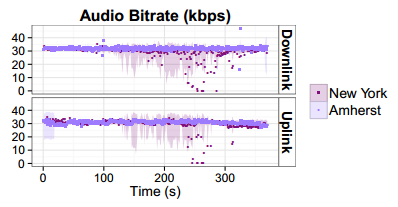
\includegraphics[scale=0.4]{mobile-audio-metrics.png}}
\caption{WebRTC audio performance shown as representative values
(points) and a range of one standard deviation above and below the
mean (shaded area).}
\label{fig:mobile-audio-metrics}
\end{figure}

An important thing to mention is that video quality is not that important when it comes to communication, the audio quality is of much more value\cite{fund2013performance}. We can observe from Figure \ref{fig:mobile-audio-metrics} that the audio bitrate is mostly consistent, degrading only in extremely poor channel quality. The biggest problem here as seen in Table \ref{tbl:wrtc-packet-loss} is that the packet loss is quite high on the uplink for audio in the urban environment. This is because the quality is not reduced to keep the audio signal clear. This could be somewhat fixed by retransmission of the packets, but this will again increse latency.
\\
\begin{table}[here]
\centerline{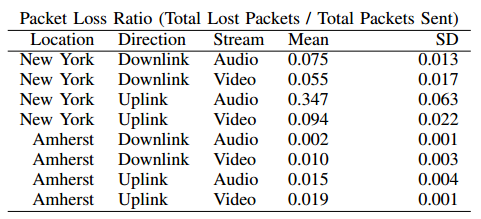
\includegraphics[scale=0.4]{wrtc-packet-loss}}
\caption{Packet loss ratio for a WebRTC session.}
\label{tbl:wrtc-packet-loss}
\end{table}

\subsection{Connectivity}
Another concern is persistent connectivity. For an app to be reachable for incoming connections, it needs some kind of persistant communication channel. Most cellular networks have a firewall preventing incoming TCP connections\cite{isomaki2012considerations}. To keep a TCP connection alive, the application needs to send some kind of keep-alive packets with a high enough frequency to avoid a connection timeout. Problem with keeping a connection open all the time is that is that device's radio will consume a lot battery. Therefore, the keep-alive packets should only be sent infrequently.

\subsection{Summary}
Most of the performance issues is handled by the underlying technologies of \gls{wrtc}, which actually is pretty good at adapting bandwidth usage in variable network conditions, but it is important to be aware of these problems when developing applications. The effect that a mobile users uplink is much worse than its downlink has great impact on a user's perception of the connection. However, the most important factor for us to consider is how we will do the signaling with a mobile device, since we can't keep a connection open all the time, as that would drain the battery.

% \newpage
% \section{Related technologies}
% There are a lot of implementations of real-time communications out on the market today. Let's take a look at similar technologies\cite{lopez_fernandez_catalysing_2013} that is in direct competition with \gls{wrtc}:

\subsection{Real-time communications}
For doing real-time communications we have commercial services such as Skype, Tokbox, and Google Hangout. 

Skype is definately the biggest one in this category. Skype utilizes peer-to-peer technology by leveraging all of the available resources in a network, this is probably why they can manage free communications. Using centralized resources is very costly. Skype has very successfully developed a video collaborations system utilizing peer-to-peer technology, but the quality depends on the users available resources. This is the same with the current networking model of \gls{wrtc}.

\subsection{Live broadcasting}
Services that does live broadcasting such as Ustream, Twitch, and Google Chromecast are also in competition with \gls{wrtc}. 

A lot of e-commerce sites are looking to integrate \gls{wrtc} as part of their customer service experience. Today it is normal to have live text chat, but with \gls{wrtc} it is easy to integrate video support as well.

In addition we have vendors providing technologies at different layers of the protocol stack such as Microsoft's Lync and Apple's FaceTime. It is also worth to mention common open source services like Asterisk\footnote{Telephony switching services} that are heavily used in commercial software. Asterisk has recently increased their signaling services to support \gls{wrtc} as well.

These companies have made significant investments to build their services, and with the introduction of \gls{wrtc} these companies are both threatened by competing businesses, but the tehcnology also opens up for new opportunities.

There exixst two public projects for doing server-side processing of media namely Tokbox and Lynckia. Righ now these services are limited to interact with other \gls{wrtc} endpoints. There is no interoperability with non \gls{wrtc} clients.

Missing technologies in \gls{wrtc} that we can find in other services, are PUSH capabilities, interop with other legacy systems such as SIP, more flexible group conversation architecture, advanced media sharing capabilities. These would require server-side capability.

% \newpage
% \section{Current implementations}
% %!TEX root = ../main.tex

There are some quite popular implementations of \gls{wrtc} today, although very few of these use \gls{wrtc} exclusively, we will mention a couple of the most popular ones, along with some platforms for simplifying \gls{wrtc}.

\subsection{Browsers}
Google's desktop and android versions of Chrome incorporates \gls{wrtc}, as does Firefox. \gls{wrtc} support on Opera is on the way. There is still uncertainty about when Internet Explorer will add support. Google and Mozilla has displayed interoperability between Chrome and Firefox. This is necessary to achieve transparency regarding the browser being used, therefore preventing the use of a particular browser. 

\subsection{Hangout}
Google's Hangout\footnote{http://www.google.com/hangouts/} is competing with Skype in the desktop videoconferencing space. Parts of the \gls{wrtc} stack is implemented in Hangout's code base, but Hangout is not a pure \gls{wrtc} implementation yet, simply because it needs to work on every browser, therefore it is packaged in a browser extension, but the underlying works relies heavily on \gls{wrtc} technologies.

\subsection{Chromecast}
Google's Chromecast\footnote{http://www.google.com/intl/en/chrome/devices/chromecast/index.html} uses \gls{wrtc} as well, but in a different way than Hangout. It is only used for one-way streaming from you device to a TV. Other services in the live broadcasting space such as Twitch\footnote{http://www.twitch.tv/} could be seeing competetion from \gls{wrtc} in the near future.

\subsection{WeCam and API platforms}
The app WeCam\footnote{http://wecamchat.com/} let's you video chat with your Twitter, Google+, and Facebook friends. It uses an API platform called OpenTok that simplifies much of the \gls{wrtc} setup, such as signaling. By leveraging platforms you suddenly get access to a lot more features on top of \gls{wrtc}, but these platforms cost money. Then again they add important functionality that's missing from \gls{wrtc}, such as being able to do processing of media. Two examples of public projects for doing server-side processing of media are Tokbox and Lynckia. Right now these services are limited to interact with other \gls{wrtc} endpoints and there are no interoperability with non-\gls{wrtc} clients. Other missing technologies in \gls{wrtc} that we can find in related services are PUSH capabilities, interoperability with legacy systems such as SIP, more flexible group conversation architecture and advanced media sharing capabilities. All of these currently require some sort of server-side architecture.

\subsection*{Summary}
\gls{wrtc} is definately on the right path to becoming big, as it's being utilized in a couple of very popular applications, but right now it's missing some key features to become a permament solution for companies. It currently acts more like a tool to simplify much of the underlying aspects of doing real-time media, you have to take care of the rest yourself. One of the big things that's missing are being able to do processing of media, however upcoming companies sell their services on top of \gls{wrtc} to allow for these features.

\newpage
\section{Background summary}
\gls{wrtc} brings a lot of new technologies to the table. It is an effective tool that can be used to quickly create real-time communication applications, with the added advantage of support for a lot of mobile devices. With the new APIs we can run a client on any tablet or mobile phone that has a web browser with support for the \gls{wrtc} standard. %Related technologies developed by Cisco and Microsoft are more complete and are now dominating the communication space, but it's going to be interesting to see if they will loose some markets to smaller companies utilizing \gls{wrtc} in the future. Google has successfully used \gls{wrtc} in their Hangout application and on their Chromecast devices. Probably the biggest problem with \gls{wrtc} right now is that the IETF working group have not agreed on a video codec yet, which is somewhat halting the development.
Visual Solutions VA application is using transport technologies that needs to have added security layers to work with \gls{wrtc} and the media formats needs to be transcoded with the appropriate codecs. Also the signaling and routing needs to be enhanced to make Virtual Arena work with \gls{wrtc}. In the next chapter we will describe the problems of integrating \gls{wrtc} with Virtual Arena.

%\chapter{Virtual Arena}
%%!TEX root = ../main.tex

\section{How can we integrate RTC in the Web with Virtual Arena?}

This chapter is about the challenges of making two different media systems work together. It will discuss a possible solution and the pros and cons of this. Then we will look at how Visual Solutions can best integrate this solution and how their vision can be solved.

\subsection{How does Virtual Arena work?}

Virtual Arena supports one-to-one, one-to-many and many-to-many collaborative scenarios. The application uses a \gls{mcu} that acts as a media server. With this server Virtual Arena can support a lot more incoming and outgoing streams than in a simple peer-to-peer scenario. It also applies mitigation strategies for scenarios with limited bandwidth. Without going into too much detail of how the application is actually put together the main setup looks something like this: 
\\
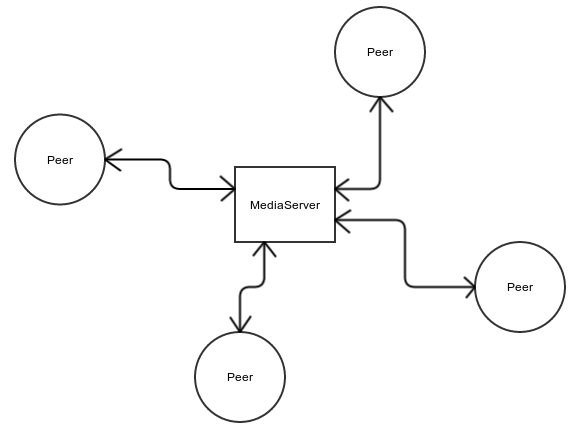
\includegraphics[scale=0.6]{mediaserver.png}
\\
\\
Communication between peers and the media server is done by opening up ports in the firewall to listen for incoming tcp and udp connections. The media server can receives incoming streams and mix it in with the other streams and forward it to all the other peers. All the streams are identified using an SSRC.

\subsubsection{Signaling}
Virtual Arena uses a proprietary way of doing signaling over RTCP.

\subsubsection{Transport}
Raw RTP stream over UDP.

\subsubsection{Media}
Speex for audio and theora for video.


\subsection{How does WebRTC work?}
WebRTC is a very complex synergy of components and protocols. But from a frontend developers point of view, all of this is packaged into three main Javascript API's: getUserMedia, RTCPeerConnection and RTCDataChannel. These are defined by the \gls{w3c}. 

The exchange of real-time media between two browsers follows a process like this:
\\
\\
1 Input devices are opened for capture as the media source. This is done using the getUserMedia API.
\\
\\
2 Now we have to signal the other users that we want to connect to them. using RTCPeerConnection we send an \gls{sdp} offer to the other clients, which generates an \gls{sdp} Answer.The \gls{sdp} here includes \gls{ice} candidates. Which opens ports in the firewall. There is a fallback if both clients are on symmetric \gls{nat}'s and a connection isn't possible to use a \gls{turn} server that acts like a packet mirror, channeling all the packets through the \gls{turn} server.
\\
\\
3 Once connection is successful, a \gls{dtls} connection is opened and all the media from input devices are encoded into packets and transmitted using \gls{srtp}-\gls{dtls} streams.
\\
\\
4 At the destination, the packets are decoded and formatted into a MediaStream.
\\
\\
5 The MediaStream is sent to output devices
\\
\\

\subsection{What are the differences?}
While Virtual Arena provides a very simple and not so secure solution media level. This because in a closed enterprised environemnt this is not needed. Most of the security will lie in the firewall anyways.

But since \gls{wrtc} is a very open solution and is supposed to work with public users firwall configurations, a lot more complex security architecture is needed.

So while \gls{wrtc} packages all their streams in a new format called a MediaStream. At the transport level everything is encrypted using \gls{dtls} on top of \gls{srtp}.

\subsection{What do we need?}
There are several problems here. Since Virtual Arena operates on a low-level not much is needed. All we need is to listen to a specific ip-address on a specific port on UDP transmitted data. In the packet headers we will find an \gls{ssrc} that we use to identify the incoming packets.

With WebRTC on the other hand, we are only allowed to work on a higher level. We cannot access MediaStreams directly without first opening a connection with another peer. This is a problem. This means that we first have to iniate a normal RTC Connection before we can look at any identifiers such as the \gls{ssrc}. We cannot listen on specific ports for incoming RTC connections, and we cannot specify a specific port to transmit data. Also as of now the current implementation of WebRTC is not designed to add local external streams to the connection. This means that getting WebRTC to work with any external application, we have create some sort of gateway server.
\\
\\
\textbf{By having done tons of experiments I propose this solution:}
\\
\\
One gateway server that can listen to UDP-packets from the Visual Solutions \gls{mcu} and acts as a peer in WebRTC. This is not an ideal approach, but the most viable at the moment. Ideally one would integrate WebRTC over the whole spectrum, which is both inconveniant and leads to complications.

For a single person that acts as a PeerConnection in WebRTC to listen in on a conversation from Virtual Arena, one would need to initiate a fake RTC Connection using two peers, then create a MediaStream from the incoming UDP packets and inject that MediaStream into the RTC Connection. On the returning side one would have to take the MediaStreams and break them into pure RTC packets with an SSRC identifier in the header and send them in return to the \gls{mcu}.

First problem is receiving the incoming conversation from Virtual Arena this can be done setting up a socket that listens for incoming UDP packets. This is not a problem and can even be done in a pure Javascript environment using node.js

Then one would have to create a MediaStream Object from these packets. This is not currently possibly using chrome API's or Firefox. In chrome it is possible to create a pure audio MediaStream using the new WebAudio API, and in Firefox it should be possible to create a MediaStream from video using getStreamUntilEnded(), but this is currently broken. In the future however this should be possible using the drafted captureMedia API.

It is however possible to inject external MediaStreams into an RTC Connection.

For returning data from a PeerConnection to the \gls{mcu} on would have to record the stream and return the data over a an \gls{udp} connection. This should be done using the proposed MediaStream Recording APIs, but none of the browser have currently implemented these yet.

\chapter{Problem Statement}
%!TEX root = ../main.tex

This chapter will describe the problems of integrating \gls{wrtc} with enterprise communication systems. It will also present the goals of doing this research, present the research question, define the research and implementation method, then lastly present the expected results.

\section{Problem Description}
The \gls{byod} policy allows workers to bring their own mobile or tablet device to work. In enterprises this policy generates a lot of problems regarding how to handle security. One thing people need is to be able to access their enterprise internal communication system from their own device. The \gls{wrtc} technology allows us to easily create mobile clients, but how do we get these to interact with existing enterprise communication systems? We need some kind of technology that interworks these two technologies. What we need is to have the underlying protocols of \gls{wrtc} work together with traditional enterprise communication protocols. We also need to have the two systems being able to communicate with each other through message exchanging and signaling. Last but probably most important is how to handle access policies and crossing the enterprise firewall. The advantages of supporting \gls{rtcweb} in enterprise communication systems are huge. Immediately the system can access any WebRTC-enabled browser. This means we can reach out to a whole range of new devices. We basically get universal mobile support, easy client integration with top security, and no need to download applications or plugins, the app runs directly in the browser.

% Doing real-time communication in the web browser is nothing new, flash implementations have existed for a long time, and Google's Hangout is quite popular, but \gls{wrtc} seems to have some important advantages over the other technologies.

% \begin{itemize}
%     \item Universal mobile support
%     \item Easy integration, with a high focus on security.
%     \item No need to download clients or plugins.
% \end{itemize}

% By looking over the drafts done by \gls{w3c}, \gls{wrtc} seems to be well suited for doing collaboration directly in the web browser.


% \section{Problem statement}
% \gls{wrtc} seems to be the best solution for doing video conferencing on the web, and both desktop and mobile web browsers have some degree of support which improves on a nightly basis.

% While other solutions like Flash may have better support at the moment, there is a clear indication that the web is moving towards open standards\cite{jennings_real-time_2013}. A lot of effort is being put into \gls{wrtc} at the moment by big companies like Google and Mozilla to create this technology, however there are still disagreements about which audio/video codecs is going to be used\cite{philippe_video_2014}.

% All the browsers that support \gls{wrtc} only support different subsets of the features specified by the \gls{w3c}. Therefore a lot of experiments had to be conducted to see what kind of features worked and which did not. It was also necessary to test different codecs, to see which ones was allowed to use in the different browsers.

% It's interesting to see if this technology is mature and usable enough to work in a enterprise environment. We also have to see what features are planned for the future of \gls{wrtc}, and if support for more platforms are coming.

\section{Research question}
This thesis will try to answer the following question:
\\
\\
\textbf{How can we best integrate \gls{wrtc} with a enterprise communication system for doing collaboration?}
\\
\\
Supporting questions:

\begin{itemize}
    \item How should we approach developing a \gls{wrtc} client for mobile devices?
    \item How will this technology improve in the near future?
\end{itemize}

By answering these questions, it will be possible for multiple businesses to take advantage of the \gls{wrtc} technology by utilizing a gateway that interoperates with their existing systems for doing communication, with the addition of some important notes on developing clients for mobile devices.

\section{Research method}
The research method used in this thesis, is a quantitative experimental method, using systematic investigation and analysis of the different implementations in browsers of the drafted APIs by the \gls{w3c}. Experiments is done to examine the actual workings of the implementations to uncover support for the protocols and codecs defned in \gls{rtcweb} by the IETF. Practical experiments are run in Chrome, Firefox, and Chrome for Android. Different SIP applications will be used to test interoperation through a gateway. Wireshark\footnote{Wireshark is a network protocol analyzer} is used to capture and analyse traffic to see what type of data is being transmitted. An open source \gls{wrtc} gateway is tested to see how well it interworks with \gls{wrtc} and other systems. 

\section{Implementation method}
A model is created to reuse as much of existing architecture as possible from the enterprise communication system. This is done to separate components as much as possible from the existing system, and thus this work extends beyond the specific industrial case in this thesis. The specifics of the industrial case will be explained further in the next chapter.



% \section{Existing work}
% There exist's a lot of tutorials on creating very simple implementations of \gls{wrtc} on the client side, usually setting up one-to-one connections using a third-party service for doing signaling. More advanced guides shows how you can setup your own server to do signaling using WebSockets\footnote{WebSocket is a protocol providing full-duplex communications channels over a single TCP connection}.

% This is great, but to be able to create an advanced server that acts like a gateway between \gls{wrtc} and Virtual Arena, we need to look further. Looking at commercial solutions that could potentially be of some help, most of them are closed. But there is one open source project named webrtc2sip\cite{doubango_telecom_webrtc2sip_2014} which acts like a gateway between \gls{wrtc} and \gls{sip} to allow a browser to create and receive calls from a legacy \gls{sip} network. It's written in C++ and it's open source, but not very well documented. It also doesn't offer exactly what we need, as it is designed to work with \gls{sip} systems. An other interesting project is an open-source \gls{mcu} called Licode\cite{lynckia_licode_2014}, this one is not designed to include external \gls{rtp} streams, but if this functionality could be implemented server side along with a proxy for doing signaling, it could be a very interesting project.

% There is no good service on the web that provides live data on how far the support has come on different browsers. There is one service that will check for WebRTC and WebSockets connectivity on \url{http://www.check-connectivity.com/}. There are blogs and articles that provide tables showing who has implemented which APIs, but most will be outdated.


\section{Expected results}

\begin{itemize}
    \item From this thesis I will have provided a model of how an enterprise can integrate WebRTC with their own communication systems. I want to provide information and guidelines about all the necessary technologies that needs to be implemented.
    \item Also I would like to provide guidelines on how to design a mobile friendly WebRTC client.
\end{itemize}


\chapter{Industrial Case}
%!TEX root = ../main.tex

This thesis is written in cooperation with Visual Solutions\footnote{http://www.bbvisuals.com/}.

Visual Solutions is a Norwegian company in the BB Visual Group\footnote{http://www.bbvisualgroup.com/} Their primary business is within the integration of operations for the oil and gas industry. They have offices in Houston, US, Brighton, UK and a headquarter in Bergen, Norway.

Visual Solutions contribute tailor made solutions enabling and improving collaboration and cross-disciplinary interaction across organisation units and geographic locations.

One of their applications Virtual Arena\cite{solutions_b2|virtual_2014} is a powerful and interactive tool that allows IP-based application sharing within collaborative sessions. Virtual Arena supports one-to-one, one-to-many and many-to-many collaborative scenarios, with support for high-performance application sharing, audio and video communication from an advanced 3D shared scene.

\section{Visual Solution's vision}
In today's  world everybody owns some kind of mobile device. If a user could enter a collaborative session from the web browser of their own simple mobile device, this would be of great benefit to the customer. The user would not have to install any additonal plugins or software to their device. Many new API's are currently being developed to improve communication and hardware access in the web browsers. The \gls{w3c} has drafted a document that defines a set of API's to allow media to be sent to and from another browser or device implementing the appropriate set of real-time protocols.

Visual Solutions wants to investigate how far development has come with these new API's and if their vision can be accomplished by using them in their application.

The problem can be defined in two sub-problems:
\\
\\
\textbf{Problem 1}\\
Is it possible to use these new API's together with Visul Solutions current application? How can these new API's be implemented with their current software solution Virtual Arena?
\\
\\
\textbf{Problem 2}\\
It is in Visual Solutions interest to gain knowledge of how good the support for these new API's are today in desktop browsers and on mobile devices. This would give an indication to whether or not there is anything to gain from investing in further development.

%\chapter{The Approach(experiments)}%
\chapter{Interoperation}
\gls{wrtc} deviates from traditional enterprise collaboration systems by opening up communications from every web application instead of controlled software pieces. So how do we make the open web interoperate with the closed enterprise world. There are two ways of going about this problem. We can either choose to redo the whole existing architecture of the enterprise collaboration system putting \gls{wrtc} technology in the center and upgrade all the existing infrastructure to support \gls{wrtc}, but this is an expensive solution, especially since the \gls{ietf} has not yet finished deciding upon which protocols and codecs to be used. Therefore, the best option is to extend current architecture with \gls{wrtc} capabilities. To do this we have to create a gateway between the underlying technologies of \gls{wrtc} specified as \gls{rtcweb} and existing enterprise infrastructure. The aim when creating a gateway between the two systems is to re-use as much as possible of existing architecture.

\section{Requirements and problems}
There are basically three planes we have to make interoperate: the signaling plane, the media plane, and the IP addressing plane. 
By signaling we mean the offer/answer exchange. The media plane is the transportation of the media, and the IP addressing plane is basically how we connect to each other.

\begin{figure}[here]
\centerline{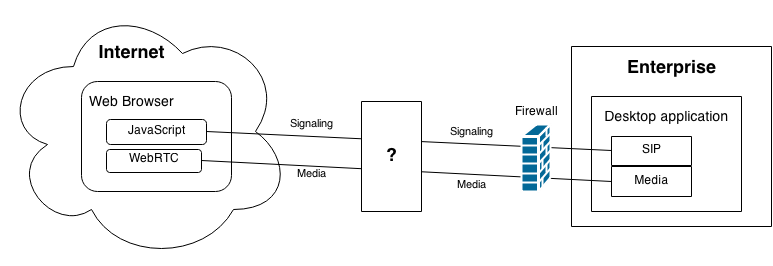
\includegraphics[scale=0.5]{gateway-layers.png}}
\caption{WebRTC-Enterprise interworking}
\label{fig:gateway-layers}
\end{figure}

\subsection{Signaling}
\gls{wrtc} does not define any standard way of doing signaling, but we do have to implement it and get it working with typical enterprise ways of doing this. In order to get a session going, the peers should only have the need to exchange four things for establishing a secure connection in addition to information about the media:

\begin{itemize}
\item{An ICE username}
\item{An ICE password}
\item{A list of possible ICE candidates}
\item{A DTLS fingerprint}
\end{itemize}

The current \gls{wrtc} specification says to exchange this information with the browser API in \gls{sdp} format. \gls{sdp} is an old format used in the \gls{voip} world, therefore the re-use of \gls{sdp} is supposed to save time, but the anatomy of an \gls{sdp} is complex and constantly changing because the \gls{ietf} are coming up with new stuff to include. All the information has to be excactly right or it will be rejected by the browser. It is highly unlikely that the current specification of \gls{sdp} will work with any older implementation found in any enterprise communication system.

Another thing is that \gls{wrtc} has to do signaling running over HTTP, while the standard in an enterprise system is to use \gls{sdp} with \gls{sip} or some other proprietary way over TCP or UDP.

We need to come up with some way of manipulating the \gls{sdp} and possibly use a \gls{sip} stack developed in Javascript running in the client.

\subsection{Media}
In the \gls{wrtc} world the media plain is designed to avoid having to relay media streams. The goal is to have pure peer-to-peer connections, while in the enterprise world it is common to have full control over the media plane and in most cases use some kind of media server. Also the \gls{wrtc} specification says that support for \gls{ice} and \gls{srtp}-\gls{dtls} are mandatory. Encryption is hardly ever used in the enterprise world, so this is another challenge. If encryption is used, it is more common to use \gls{srtp}-\gls{sdes} with the keys being handled on the signaling plane, rather than in media plane that is the case with \gls{dtls}.

\gls{wrtc} uses one-way media streams, while an enterprise system usually expects to receive bi-directional streams. This can be fixed by multiplexing the streams, so we can have multiple streams running over the same network port.

The biggest issues here is probably which codecs we need to implement. The \gls{ietf} has landed on two default audio codecs, but has not decided on which video codec to use yet. The most typical enterprise video code used is H.264. Right now the \gls{ietf} are deciding between VP8 and H.264, so currently we have to support both and do server side transcoding between them.

\subsection{IP addressing}
In the enterprise world a \gls{sbc} is commonly used to control incoming media traffic. In \gls{wrtc} one uses \gls{ice} browser-to-browser to cross firewalls. We have to handle both exchanging of \gls{ice} candidates and bypassing the enterprise firewall. This is a bigger topic that we will go more deeply into in the next chapter.

\section{Summary}
The first iteration of \gls{rtcweb} is still under development, and not all protocols and codecs have been decided yet. It is theoretically possible to create a gateway and it has been done before under closed doors. Some of the biggest issues are how to handle the signaling, translating the media, and crossing the enterprise firewall. In the next chapter we will further look into how to traverse the enterprise firewall before we finally introduce a solution to the problem.


\chapter{Enterprise and Firewalls}
\section{Enterprises and Firewalls}
Enterprise software enable multiparty conference scenarios within a guarded enterprise network. Usually with a session-centric client-server architecture. Enterprise communication software usually uses an \gls{sbc} to communicate with the outside world. \gls{wrtc} is not designed to work with current \gls{sbc} deployments. We look into how we can adapt an enterprise firewall to work with WebRTC.


\subsection{Firewall}
Enterprises use firewalls to enforce Internet Protocol access policies at the edge of their networks. These policies relate to who is allowed to access which resources. The firewall are often implemented using 5-tuple rules (source and destination IP address, source and destination ports, and transport protocol). Typically firewalls were developed to handle client-server protocols such as web browsing, email, and file transfer\cite{johnston_taking_2013}. Peer-to-peer communication systems are bigger challenges to firewalls, and since \gls{wrtc} is designed to work peer-to-peer, this introduces some problems. \gls{rtp} packets are typically described as peer-to-peer flows. Media can be sent from inside the firewall, but the reverse flow often gets blocked. This is why \gls{ice} was developed, to make firewall traversal easier. But enterprise communication software usually has a client-server architecture, to communicate with entities outside the enterprise network, it is common to use a \gls{sbc}. Currently \gls{sbc}s won't work well with \gls{wrtc}. This raises some questions:

\begin{itemize}
\item How can the enterprise firewall adapt to WebRTC?
\item How can the enterprise firewall detect and apply policy to WebRTC flows?
\end{itemize}

\subsection{Session Border Controllers}
An \gls{sbc} is essentially an application layer firewall with a signaling and media application layer gateway built in. The \gls{sbc} is usually connected in an enterprise demilitarized zone(DMZ) as a trusted enterprise network element. It blocks all unauthorized signaling and media flows, and provides a point of policy enforcement as shown in Fig\ref{?}. As specified by IETF\cite{sbc} a \gls{sbc} should support \gls{sip}, \gls{rtp}, and \gls{srtp}. \gls{sip} is a signaling protocol used for VoIP and video communications to establish RTP media sessions. By parsing SIP messages, the SBC is able to discover the transport addresses (5-tuple) to be used for the media session. The \gls{sbc} opens a filter rule permitting the \gls{rtp} traffic, and the RTP media session is able to traverse the firewall. Since SBCs are widely deployed it makes sense to reuse them for WebRTC. However, there are problems with this approach. WebRTC has no concept of sessions; instead, it has a concept of `streams'. Streams have media sources and sinks that generate and consume media flows. One possible apporach would be to translate every WebRTC session that crosses enterprise boundaries into a communication session that its existing infrastructure could handle in a session-centric manner. This could mean converting a WebRTC session into a SIP session, then converting back again.

The SBC should either be upgraded to support WebRTC or we should opt for another way of detecting WebRTC flows.

\subsection{WebRTC Firewall Traversal}
If upgrading the SBC is not trivial, we can look at the other planes for detecting an incoming WebRTC session:

\subsubsection{ICE}
There is a standard type of signaling protocol used for establishing media flows as part of WebRTC. It is built into the ICE protocol used for traversing firewalls. Before any media flows, ICE is run between two browsers. This could be used to detect an ICE exchange starting up across the enterprise border. This could then be used to distinguish a WebRTC media flow across the border, allowing policy to be applied.

\subsubsection{SRTP}
Another approach might be to use SRTP key negotiation along with \gls{dtls} to authenticate the media flow. For example, since SRTP-DTLS is used for key management, the secure edge could act as a man-in-the-middle an hence validate the public key in the fingerprint. A self-signed key from the browser could be stored in an enterprise key server. This could allow the secure edge to authenticate the browser inside the enterprise network and apply appropriate policy.

\subsubsection{Media Relay}
Another approach would be to require a media relay to be used for \gls{wrtc} media sessions crossing the enterprise boundary. There is a standard protocol for this relay, known as \gls{turn}. The enterprise firewall would be configured to block non-relayed \gls{wrtc} media flows. The enterprise would then deploy a \gls{turn} server in the \gls{dmz}, and permit media flows that go through this server. During media flow setup, the TURN server could authenticate the user and also learn what type of media flow is to be set up based on the bandwidth requested. Policy could then be applied to this media flow.

\subsection{Summary}
Doing peer-to-peer communication crossing enterprise networks are difficult. It might not be trivial to upgrade current SBC implementations, therefore we looked into other ways of detecting WebRTC traffic for applying policy to the media flows. In the next chapter we will look at the other challenges of integrating WebRTC with enterprise communication software. 

\chapter{WebRTC for Mobile}
%INTRO
When developing a \gls{wrtc} client for mobile devices there are two ways to go about this. Either create a HTML5 app or embed \gls{wrtc} into a native app. \gls{wrtc} itself provides a high-quality media engine for voice and video that adapts to network conditions automatically. Security is high due to encryption of media packets. But using the javascript APIs or some third-party SDK is one thing, we still have to create a way of doing signaling ourself, since this is not standardised yet. Creating a client that works for mobile phones is beneficial for the \gls{byod} policy of permitting employees to bring personally owned mobile devices (tablets, smart phones) in enterprises.

\begin{quote}
``Enterprise migration toward tablets from PCs will effectively cause many - if not most - companies to `dismantle' their current business-as-usual approach to technology'' - Eric Schmidt
\end{quote}


\section{Mobile client for WebRTC}
When developing a client for our mobile devices there are a few options. For Android we have advanced implementations of \gls{wrtc} directly integrated in both the chrome and firefox mobile browsers. But for iOS we have to use third-party SDKs to embed \gls{wrtc} into a native app.
Using a web browser application is great for when the user has a planned meeting, this way he can open or join an ongoing session, but the user will not be available to receive incoming calls. It migh be benficial to create native applications on mobile phones to allow for receicing messages of incoming calls.

A few the problems specific to mobile devices are bandwidth usage, CPU and power limitations, signaling, and sound echo.

\subsection{Bandwidth}
Mobile bandwidth usage comes at a premium, and \gls{wrtc} dynamically adjusts each stream for maximum bandwidth usage at best quality. There is not much we can do about this on the client side, but we could be able to transmit lower bandwidth video if we used a media server for manipulating the media before it's transmitted. 


\subsection{Processing}
The encoding and decoding of video is CPU expensive. The H.264 codec is the most CPU friendly one, since it has a greater range of devices supporting hardware acceleration. But in this day and age, this is a minor issue that will soon become irrevelevant due to the rapid increase in mobile processing power we're seeing. A bigger issue are multiparty streams since software encoding barely supports single streams, so for multiple streams we have to use server side mixing of the streams to have support for multiparty sessions.


\subsection{Signaling}
The mobile radio is one of most battery draining units on our mobile phones, so we need think about how we do our signaling, since keeping an open connection all the time is very expensive. The main issue here are how to listen for incoming connections, when we are actively using our app its natural to keep an open socket all the time, but when we are not actively using the phone, it might be better to listen only infrequently for incoming calls or opening up a socket when receiving a push notification notifying the user of an incoming call. Both Google's Cloud Messaging (GCM) service and Apples's Push Notification Service (APNS) allows for persistent connections, which will allow for the user of an application that is not running to be alerted that the application has data waiting for it.


\subsection{Echo Cancellation}
The biggest issue relevant to a user is call quality. When the microphone is placed near the speaker a common problem is echo, this happens when the microphone records output from the speaker. This may not be audible for the user, but can be very annoying for the other party. The solution here is to use echo cancellation techniques. This is integrated in the \gls{wrtc} audio engine, but currently it works poorly on mobile devices. The technique used is \gls{aec}. It works by analyzing the sound output being played from your speakers and removes it from the sound captured by your microphone. But lots of Android devices are unable to handle \gls{aec}\footnote{https://code.google.com/p/webrtc/issues/detail?id=2580}. The lazy solution is to recommend the user to use earplugs/headphones so that the microphone cannot pick up sound from the speakers. The advanced solution would be to implement third-party echo cancellation software specialized to each platform and device.


\section{Summary}
When developing \gls{wrtc} clients for mobile devices, we have to think about a lot of problems specific to mobile devices in contrast to desktop clients. Specifically processing limitations for multiparty sessions, we should use a mediaserver to mix everything into single streams that are easier to process. Battery consumption when doing signaling can be fixed by utilizing push notification services. And echo noise issues are easily avoided by using a headset until the \gls{aec} for mobile devices improve.

%\chapter{The Implementation(how implemented approach)}%
\chapter{Integration}
In this chapter we will explore the technical requirements for integrating \gls{rtcweb} with an enterprise communication system architecture and give the suggested solution along with discussing some of the problems raised by the integration.

\section{Integration}
There are basically two ways of going about this problem. The first would be to directly integrate \gls{wrtc} in the enterprise architecture. We could then use SIP-over-WebSocket signaling and use an end-to-end media path enabled by \gls{wrtc}. This could work if the legacy enterprise system supported all the required protocols defined in \gls{wrtc}, otherwise the architecture would have to be upgraded to support all the new features. This is not trivial, since it would require to redo all of the existing architecture just to support \gls{wrtc}. It is better to create a bridge in the form of a gateway between \gls{wrtc} and the legacy architecture.

\subsection{The Gateway}
First showing a simple web application P2P WebRTC structure. Here signaling goes through a signaling server and media travels directly between the two peers(browsers). A STUN server is used for receiving ICE candidates, if that fails there is a fallback transporting media through a TURN server.
\\
\begin{figure}[here]
\centerline{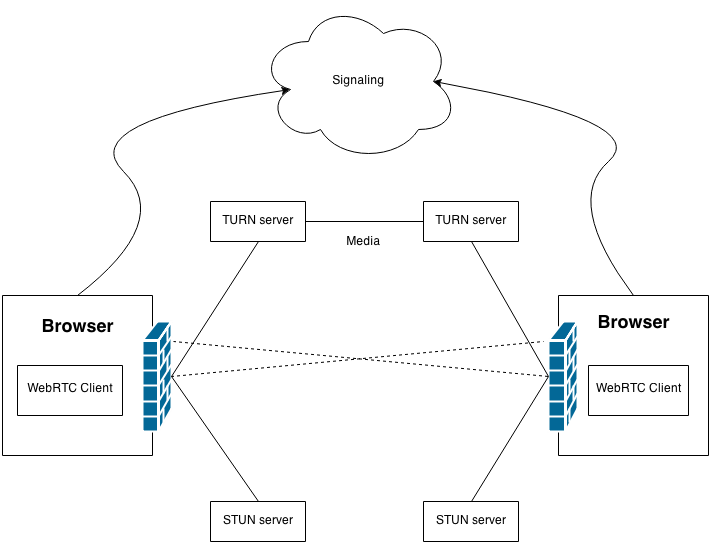
\includegraphics[scale=0.35]{webrtc-p2p-architecture.png}}
\caption{WebRTC P2P architecture}
\label{fig:jsep}
\end{figure}

Secondly showing a typical enterprise architecture with a signaling server, media server, and a server for routing the streams to peers.
\\
\begin{figure}[here]
\centerline{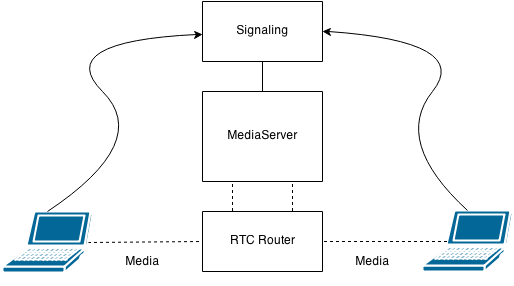
\includegraphics[scale=0.45]{enterprise-mcu-architecture.png}}
\caption{Enterprise communication platform architecture}
\label{fig:VirtualArenaArchitecture}
\end{figure}

Let's see how RTCWeb can be used to connect to existing enterprise communication networks. In the solution figure we add an interworking gateway component. This component includes three subcomponents:

\begin{itemize}
\item{Signaling Proxy}
\item{Media Transport Proxy}
\item{Media Transcoder}
\end{itemize}

These components should provide all the necessary functionality we need.
\\
\begin{figure}[here]
\centerline{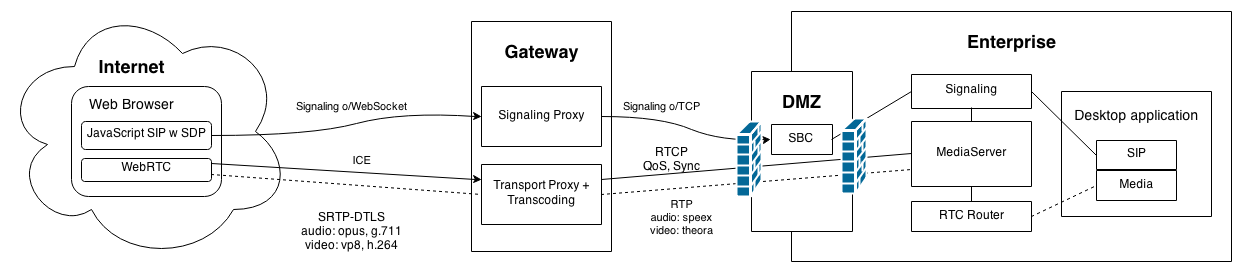
\includegraphics[scale=0.40]{gateway2.png}}
\caption{WebRTC-Enterprise Gateway}
\label{fig:wrtc-enterprise-gateway}
\end{figure}

\subsection{The Signaling Proxy}
In this implemenation the client has implemented signaling using a \gls{sip} stack in Javascript. The SIP includes the \gls{sdp} and this is transmitted over HTTP using WebSockets. Then the signaling proxy will manipulate the \gls{sdp} to support the enterprise implementation of \gls{sip} or any other proprietary way. The SDP would also only include TURN addresses so we make sure that the media always gets routed through th e gateway, blocking all other candidates. The message would then be transported through the enterprise \gls{sbc}. The Signaling proxy has to generate an offer for the client, then on the client the remote party would install it using the setRemoteDescription() API.

\subsection{The Transport Proxy}
The \gls{wrtc} specification make support for \gls{ice} and \gls{srtp}-{dtls} mandatory. The problem here is that our enterprise architecture uses raw \gls{rtp} streams, it does not need the added transport layer security that \gls{wrtc} defines, becuse of its strict firewall policies. It is up to the Transport Proxy to convert the media streams to allow these two worlds to interoperate. The Transport Proxy also has to function like a TURN server, this so we can route the media through our gateway. The Transport Proxy handles the ICE connectivity checks, which in this case would only serve the address of our Transport Proxy. We do this by modifying a constraint in the IceTransport object on the client.

\subsection{The Media Transcoder}
The \gls{wrtc} specification defines these mandatory codecs:
\begin{itemize}
    \item Audio: opus and g.711
    \item Video: ?
\end{itemize}

There are still discussions on the topic of which video codec should be standard. The choice is between VP8 and H.264. The H.264 codec was recently made free by Cisco, so now both choices are royalty free. H.264 is the most widely deployed and currently has the best hardware support, but both Google and Firefox has decided to use VP8 in their WebRTC implementations. However, the Bowser browser created by ericsson for iOS, has only implemented support for h.264 in their WebRTC solution.

Our enterprise applicaton uses Speex for audio and Theora for video. So these would have to be transcoded to the appropriate formats. This is one of the advantages of creating a media transcoder because you can add support for both H.264 and VP8 and be able to create a session between Chrome, our enterprise software, and the Bowser browser on iOS. Problem with this component is that it's expensive in terms of processing and it may cause some delays in the stream.

\section{Summary}
The first iteration of RTCWeb is still under development, and not all protocols and codecs have been decided yet. It is theoretically possible to create a gateway and it has been done before under closed doors for similar systems. Some of the biggest issues are how to handle the signaling, translating the media, and crossing the enterprise firewall. The interworking efforts at the media level are expensive, and \gls{sdp} handling can be quite complex, as it will probably require remapping of its properties.

\chapter{Testing}
%\input{}

\chapter{Evaluation \& Guidelines}
%describe how you evaluated to show that your approach was successful. You may need a methods section, a results section and a conclusion

This chapter reflects on the theoretical architecture created in the previous chapter. I will break down each component of the gateway and test individual functionality using available open source tools. Secondly I will compare my model against a study 3GPP\footnote{http://www.3gpp.org/} did on giving \gls{wrtc} clients access to \gls{ims}, which is similar to this case. Then I will discuss the results and derive some guidelines.

\section{Evaluating the proposed gateway}
In this section a lot of experiments were conducted using sipml5\footnote{http://sipml5.org/}, which is an open-source HTML5 SIP client using \gls{rtcweb} for the media stack. It uses a SIP proxy for translating the signaling, a RTCWebBreaker to convert the media streams, and a media coder for transcoding. It operates very similar to my proposed architecture. In addition to that it connects to any SIP endpoint directly from the browser.

\subsection{The Signaling proxy}
In the signaling component a proxy solution was proposed to use a SIP stack for Javascript running over WebSockets. Using sipml5 and a range of different desktop SIP clients I tested to see how well the SIP proxy worked.   

\begin{table}[h]
\resizebox{\textwidth}{!}{%
\begin{tabular}{|p{1.3cm}|l|l|p{4cm}|p{4cm}|p{5cm}|}
\hline
SIP desktop clients & Audio & Video  & Latency                                                                                         & Quality                                                  & Comments                                                                                                            \\ \hline
Ekiga               & g.711 & failed & none                                                                                            & good audio quality                                       & did not get video working                                                                                           \\ \hline
Zoiper              & g.711 & vp8    & none for audio, video took approximately 5 seconds to appear, but then it was a live connection & good audio quality, huge packet loss on the video stream & crashed after just a few seconds during video conference                                                            \\ \hline
Jitsi               & g.711 & failed & none                                                                                            & good audio quality                                       & connection failed every time the application tried to negotiate a video codec, but worked fine when disabling video \\ \hline
Blink               & opus  & failed & none                                                                                            & good audio quality                                       & did not get video working                                                                                           \\ \hline
\end{tabular}
}
\caption{SIP desktop client interaction with web client using proxy and RTCWEB}
\label{tbl:sip-client-webrtc-interaction}
\end{table}

In figure \ref{tbl:sip-client-webrtc-interaction} the audio and video columns refer to the mutually agreed upon codec to be used during the signaling process. Since g.711 is the most preferred codec to be used in \gls{voip} systems it is natural that audio most often defaults to this codec. Experiments with video conferencing was not very successful, it was difficult getting a normal video session to work for various reasons, one of them being a mismatch in the \gls{sdp} which was noted in the interoperation chapter as a probable outcome. The one desktop client that did manage to get a working video session using the vp8 codec had a very high packet loss as seen in figure \ref{fig:wireshark-sip-call}. Reasons for this is hard to say as the experiment was done on a really good connection.

\begin{figure}[here]
\centerline{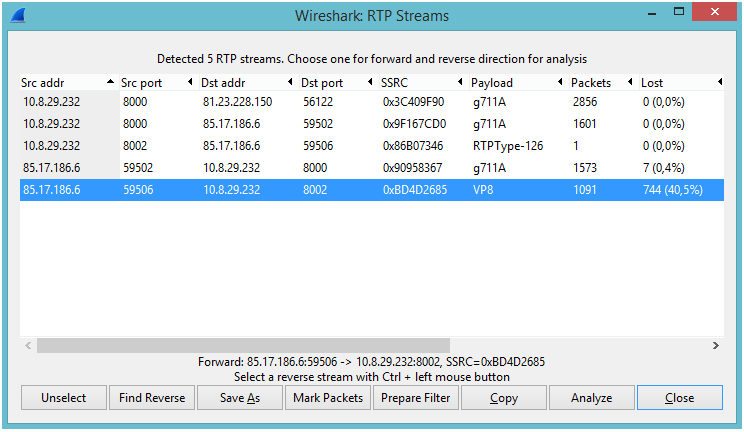
\includegraphics[scale=0.5]{wireshark-rtp.png}}
\caption{Wireshark analysis of a SIP call}
\label{fig:wireshark-sip-call}
\end{figure}

\subsection{The Transport Proxy}
Not much problems here, the connections were smooth with low latency even running behind a proxy. As mentioned earlier there was no problems doing audio calls, but video calling seemed to cause some problems, but these are probably not related to this component.

%%FYLL UT %%

\subsection{The Media Transcoder}
Since transcoding can be done in the cloud, the quality should not really be affected by this component. It is limited by which codec and your geographic location.

%%FYLL UT%%

\section{Evaluate against criteria defined by 3GPP}
What is IMS?

Why IMS? Almost all telco companies are exploring ways to provide webrtc-based access to legacy infrastructure/services they already have in palce.
These existing real-time communciation systems is or will be IMS based in most cases.

The 3gpp has started the technical definition of a solutuion for a webrtc client to access ims networks through the internet

This diagram depicts the reference architecture adopted:
3gpp tr 23.701 \ref output to date. work in progress

\begin{figure}[here]
\centerline{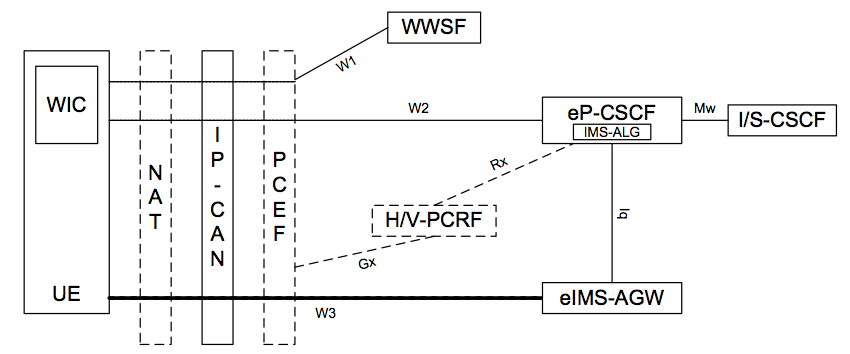
\includegraphics[scale=0.5]{3gpp-wrtc-ims-architecture.png}}
\caption{WebRTC IMS architecture}
\label{fig:wrtc-ims-architecture}
\end{figure}

Let's look at the main elements:

\textbf{WebRTC IMS Client (WIC)}
is downloaded from the wwsf. provides the aplpication logic and webrtc api calls to access communication services of ims. work on any device supproting a browser that supports webrtc.

\textbf{User Equipment(UE)}
UE device or applicationn can be a web application running on a browser.

\textbf{WebRTC Web Server Function (WWSF)}
from where the web client is downloaded.
or web server hosting the wic

\textbf{P-CSCF enhanced for WebRTC (eP-CSCF)}
entry point of SIP requests. add capacity to receive SIP over WebSockets
works as the signaling gateway. adapts signaling ont he webrtc side to standard ims-sip

\textbf{IMS Access Gateway enhanced for WebRTC (eIMS-AGW)}
supports webrtc media as defined by ietf
essentially the media gateway function.
supprot
dtls.-srtp    sdes is used in ims w keys in the signaling plane
auido/video transcoding  h.264 is supproted by h.264
rtcp multiplexing webrtc supports multiplexing of audio/video calls and rtp/rtcp over same rtp session and port. not supported in ims. must support demultiplexing

must also support negotiating ice candidates including stun and turn

the specification is open to the use of different protocols.

\textbf{IP Connectivity Access Network (IP-CAN)}
IP network used to reach the IMS core from the UE. Can be LTE for mobile, DSL and WLAN

\textbf{Policy and Charging Rules Function (PCRF) and Policy and Charging Enforcement Function (PCEF)}
supports policy and charging control decisions based on session and media-related information obtained from the P-CSCF.
Used deep packet inspection and decides based on rules whether the traffic is allowed or not.

\textbf{Network Address Translation (NAT)}
The WIC would noramlly be behind a NAT element so a box has been included in the diagram. ICE is used to enable two-way flows of srtp nehind nat so media gateway is used to exchange media flows with the ims core must support it.


\section{Results}
%Derived guidelines
this section presents guidelines and general recommendations on implementing the gateway


sip does not winterwork very well
almost all cases the sdp was the point of failure
or therer could be an agremement on an appropriate codec

\section{Conclusion}
%Peke på veien videre for å få verifisert dine anbefalinger - lead into future chapt

\chapter{Discussions and Conclusion}
%SUMMARIZE THE THESIS AS A WHOLE AS IN INTRODUCTION. DESCRIBE HOW EVALUATION REVEALED THAT YOUR SYSTEM IS SUCCESSFUL. DESCRIBE FUTURE WORK IN THIS AREA WHAT CONTRIBUTIONS HAVE BEEN MADE????

%INTRO
This chapter starts by discussing the the validity of the solution. Then present some thoughts about the conclusions, follwed by suggestions for future work.

With greatly increased number of smartphones and tabelts in the market, with different operating systems and browsers, it has become important to fin a unifying way to create content that works equally on across all platforms an screen dimensions.


%VALIDITY

%External validity
is concerned with whether the results of the research are applicable outside the context of this thesis. Whether they can generalized to a broader audience.

The industrial case provided
has both strengths and flaws with respect to validity

The goal was to find out how to interwork RTCWEB with Virtual Arena. Ericsson was the first to supply a webrtc gateway, and now the market is actually really crowded, however most of the implementation are based on SIP and IMS systems. There a couple of open-source gateways that i've found but they also only work with SIP systems and are poorly documented. The process of creating a gatewat is very similar to that you will find of IMS SIP implementations, even if pracically the individual steps are different. The goal remains the same.

Our solution is more extensive than the open-source solution, the open-source solutions does not take into consideration an enterprise firewall, nor

This thesis also expands on some of the problems of creating a client for mobile devices.

The guidelines derived are very general, and i have expanded upon the topic because i wanted my work to reach further than just a single industrial case. The focus was on utilizing exisitng architecture
The aim was to be pragmatic so as to be relevant for businesses, I believe the results do provide useful information that will be of aid when deciding how to approach this problem.

%Validity of the approach
A question that desverves attention is whether this solution is the best solution without having tested ona prototype. I believe this, because I frist drafted my model, than I found related work that looked greatly similar in nature. I refined my approach and expanded on a few areas.


%Summary and Conclusions
The aim of this study was to develop a model for an enterprise communication system could interoperate with RTCWEB. Two objectives were identified in order to achieve this aim.????

Further expanion on the problem. What was created. How was the solution validated.

Key takeaways

%Future Work
an actual implementation of the gateway modeled. Peraphs loooked into how to handle uuids. and expanded the model to work with datachannels as well.

Also my work will have ro refined as the IETF and W3C expands and changes things on a frequent basis.


%Closing remarks
WebRTC and rtcWeb is a very hot topic these days, it was really hard to find any relevant source materials in the beginning of my research, so it was a slow process in the beginning. Then suddenly the interest for webrtc exploded and several books came out explaining the different protocols and technologies. But Webrtc is continusly being develoeped. The interest is very high at the momen, and it seems that everyone you ask in the teclo busines is working on webrtc on way or another. Within a couple of years, the communicatins landscape may be totally different than what we see today.

% BIBLIOGRAPHY %
\newpage
\bibliographystyle{plainnat}
\bibliography{bibliography.bib}

% END SECTION %
\begin{appendices}
\newpage
% APPENDIX GOES HERE %
\end{appendices}


\end{document}